\chapter{语法检查}

\begin{introduction}
    \item 建议认真阅读Yx的代码和Tutorial.md。
    \item 一些建议:多和同学、助教交流。
\end{introduction}

% \noindent
% (先写一点备注) \\
% 1. 强烈建议认真阅读Yx的代码和Tutorial.md。 \\
% Yx是一个比Mx更加简单的语法,阅读Yx的实现对于代码的完成非常有帮助。\\
% Yx的github地址:https://github.com/ZYHowell/Yx \\
% 2. 一些建议:多和同学、助教交流;没有头绪时多看看Yx和学长学姐的代码,有助于理解并提高效率;
% 切忌抄袭。\\

\section{语法检查摘要}
语法检查阶段需要完成词法分析、语法分析、语义分析。在本作业中,词法分析和语法分析可以使用现有的分析库将源代码转换为语法树。
随后,你可以将语法树转换为抽象语法树从而更好地表达代码的结构。本阶段的最后一步需要你在树(语法树和抽象语法树均可)上进行语法检查(例如:简单的类型检查、if/while/for等语句的表达式合法性等),确保代码符合规则。

接下来,我们将首先讲解对于semantic阶段工作的整体理解,再对具体的实现步骤逐步解析。

\begin{remark}
    \textbf{本章节的示例为语言为Java,语法分析器为ANTLR。}
\end{remark}

\section{总览}
语法检查阶段的难点都与AST有关,分别是如何构建AST以及如何在AST上遍历进行语法检查。两个步骤的难点主要在工程实现。
ANTLR能够将我们编写的语法规则(g4文件)生成对应的parser和lexer,并构建一棵语法树。ANTLR为这棵语法树提供了Listener和Visitor的借口,便于我们提取其中的信息,
我们希望能够自定义树的每个结点,并储存需要的信息。因此,我们将继承ANTLR生成的Listener或Visitor,通过遍历语法树构建一棵抽象语法树(AST)。
最后,在抽象语法树上进行遍历,对源代码的语法进行检查。

分步骤来看,这个阶段你需要完成的任务有:
\begin{enumerate}
    \item 为语言编写文法分析文件(g4文件);
    \item 继承ANTLR生成的Visitor或Listener实现对ANTLR的语法树遍历,并同时构建抽象语法树(可选);
    \item 遍历语法树或抽象语法树对源代码进行语法检查。
\end{enumerate}

% 一份Mx代码将被转换成一棵AST,这棵树从RootNode开始,随着树的层数的加深,
% 每层的结点所表示的单位逐渐变小。下面是基于Mx的一个AST层级的简单示意:
% \begin{lstlisting}
% RootNode 
% - VariableDef
% - ClassDefinition
%     - VariableDefinition
%     - FuncDefinition
% - FunctionDefinition - Statements - Expressions 
% \end{lstlisting}

% Mx语言下,对这个结构进行一点简单的注解:\\
% 1. RootNode从全局作用域开始。Mx的全局作用域中只存在全局变量、类定义、全局函数三种类型。\\
% 2. 类定义中,只存在变量和函数。 \\
% 3. 一个函数包含多个statement(语句)。在AST中,一个函数中的每个statement都是这个函数节点的子节点。
% statement有许多种类型,比如if语句、循环语句(for、while)等等。\\
% 4. expression(表达式)有许多种类型,比如基本表达式(primary)、常量表达式(constant)、赋值表达式(assignment)等等。 \\
% 5. 关于Mx所使用的statement和expression,Mx文档中均有明确的规定,概念模糊的同学可以先仔细阅读。 \\

% 如果你对以上结构感到费解,可以仔细阅读Yx库中的g4文件(Yx/src/parser/Yx.g4)辅助理解,或者继续阅读下一部分中对于如何构建AST的详细介绍,
% 准确地理解AST的结构将会大大提高效率。\\

% \section{实现方法概述}
% 在这一部分,我们将逐任务剖析如何完成语法检查阶段。

\section{语法分析}
\subsection{语法描述文件}
我们采用ANTLR构建语法树,我们需要先写一个Mx.g4文件,用来描述Mx的语法。在这里我们以Yx-Compiler% Cite: 庄老师的repo
为例子讲述如何撰写一个ANTLR下的语法描述文件。

首先我们需要定义词法,以下的代码将\texttt{int}字符串识别为Int,将整数(以1-9开头且以0-9为后续字符的字符串、字符0)识别为DecimalInteger(思考:这里如果要支持小数该怎么写呢?)。
词法规则是有顺序的,在下面的例子中,\texttt{int}既可以是Int,也可以是Identifier,但我们只希望它被识别为Int,所以我们将Int写在前面。
\begin{lstlisting}
Int : 'int';
DecimalInteger
    : [1-9] [0-9]*
    | '0'
    ;
Identifier : [a-zA-Z] [a-zA-Z_0-9]*;
\end{lstlisting}



撰写完成词法规则之后,需要撰写对应的语法规则。
在介绍这部分之前,我们先对语句类型进行简单的划分。
一个函数包含多个statement(语句),statement有许多种类型,比如if语句、循环语句(for、while)等等。
注意,书写这部分之前,需要先对抽象语法树上可能存在的节点有个大致的规划。一般地,我们会设计Statement抽象类和Expression抽象类。
所有具体的语句都继承Statement,各种具体的表达式都继承Expression。
而针对具体的语句,需要根据语法定义要求规划节点类型。
例如,对if语句(IfStmt)节点,需要包括一个表达式节点(ExpressionNode)表达条件,两个语句(Statements)分别代表条件为真(True Statement)或假(False Statement)的语句。

以Yx的Statement部分为例:
\begin{lstlisting}
statement
    : suite                                                 #block
    | varDef                                                #vardefStmt
    | If '(' expression ')' trueStmt=statement 
        (Else falseStmt=statement)?                         #ifStmt
    | Return expression? ';'                                #returnStmt
    | expression ';'                                        #pureExprStmt
    | ';'                                                   #emptyStmt
    ;
\end{lstlisting}
在这部分代码中,定义了statement包括ifStmt、returnStmt等几种Statement,而ifStmt中表达式节点将会被解析为expression(在ANTLR的Visitor中为visitifStmt函数的\texttt{ctx.expression()}),另外两个Statement将会被分别解析为\texttt{trueStmt}和\texttt{falseStmt}。


当你完成词法和语法对应规则的书写之后,语法描述文件的实现完成。以下是一些小贴士:
\begin{enumerate}
    \item 对于Mx,如果觉得Lexer和Parser置于同一文件中过于复杂,可以考虑分为两个文件(MxLexer.g4, MxParser.g4)来书写。
    \item 如果你使用IDEA,可以基于你写的g4文件,输入一段Mx代码,可视化地生成解析树。效果大致如下,具体方法可自行查阅。
    \item antlr4的其他详细内容,请参照《antlr4权威指南》。
\end{enumerate}

\begin{figure}[htbp]
    \centering
    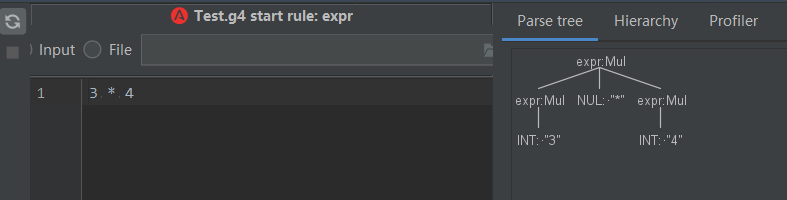
\includegraphics[width=0.7\textwidth]{image/g4.png}
    \caption{样例}
\end{figure}




\section{抽象语法树}

将撰写的g4文件传递给ANTLR后,ANTLR会生成以下文件(以Yx为例):
\begin{enumerate}
    \item \texttt{YxLexer.java}: 词法分析器。
    \item \texttt{YxParser.java}: 语法分析器,用于生成语法树。
    \item \texttt{YxBaseListener.java}: Listener类,用于遍历语法树。
    \item \texttt{YxBaseVisitor.java}: Visitor类,用于遍历语法树。
    \item \texttt{YxListener.java}: Listener接口。
    \item \texttt{YxVisitor.java}: Visitor接口。
\end{enumerate}
Listener和Visitor是antlr4提供的两种遍历方法。两者的具体意义《antlr4权威指南》(49页起)有详细说明。
这些Listener和Visitor可以被用于遍历语法树。在此之前,我们先调用如下代码让ANTLR构建语法树,\texttt{parseTreeRoot}即为语法树的根节点。
\begin{lstlisting}
YxLexer lexer = new YxLexer(CharStreams.fromStream(input));
lexer.removeErrorListeners();
lexer.addErrorListener(new YxErrorListener());
YxParser parser = new YxParser(new CommonTokenStream(lexer));
parser.removeErrorListeners();
parser.addErrorListener(new YxErrorListener());
ParseTree parseTreeRoot = parser.program();
\end{lstlisting}

\begin{remark}
    ANTLR在lexer和parser的过程中,能够发现词法、语法错误,而具体的异常类可以自定义。\textbf{并不是所有ANTLR抛出的错误都是需要处理的错误。}具体请参考Yx对于YxErrorListener类的处理。
\end{remark}

\subsection{AST节点}
现在,我们可以通过parseTreeRoot得到语法树的根节点,并建一棵AST。那么首先,我们需要为每一个节点定义一个类,来保存各自需要的信息,
从而构成一棵树。这里的树形结构和g4的语法结构本质上是一致的。
以下是Yx给出的ifStmtNode类的定义作为例子:
\begin{lstlisting}[language=Java]
abstract public class ASTNode {
    public position pos; // 用于存储节点所指代的对源代码范围
    public ASTNode(position pos) {
        this.pos = pos;
    }
    // 每个ASTNode都包括一个accept方法,可以用来遍历AST
    abstract public void accept(ASTVisitor visitor);
}
// Statement的抽象类,所有的Statement继承自这个节点。
// 同时这个节点也是ASTNode的派生类。
public abstract class StmtNode extends ASTNode {
    public StmtNode(position pos) {
        super(pos);
    }
}

public class ifStmtNode extends StmtNode {
    ExprNode condition; // 用于存储Expression(条件)
    StmtNode thenStmt, elseStmt; // 分别用于存储上文的trueStmt和falseStmt
    public ifStmtNode(ExprNode condition, StmtNode thenStmt, StmtNode elseStmt, position pos) {
        super(pos);
        this.condition = condition;
        this.thenStmt = thenStmt;
        this.elseStmt = elseStmt;
    }
    
    // 继承ASTNode的accept方法,将会跳转到对应的ASTVisitor进行节点访问。
    @Override
    public void accept(ASTVisitor visitor) {
        visitor.visit(this);
    }
}
\end{lstlisting}

需要注意,在定义AST节点的过程中,对于表达式节点(ExprNode),我们还需要关注它的类型(type)。在Mx语言中,
允许出现的类型除了Mx文档提到的int,bool等基础类型外,
还会出现Mx代码中自定义的类,所以我们需要建立一个type system来管理各种类型。
表现在具体的代码中,即ExprNode类中会含有一个Type型的成员变量,用来表示这个表达式对应的类型。(如下所示)
\begin{lstlisting}[language=Java]
    public abstract class ExprNode extends ASTNode {
        Type type;
        public ExprNode(position pos) {
            super(pos);
        }
    }
\end{lstlisting}
对于Type类,这是需要自主实现的一个类,用来根据具体的需要处理类型相关的问题(比如如何表示自定义类、如何处理数组问题等等),
Type类的实现可以参考Yx和他人的代码。


\subsection{构建AST}
ANTLR生成的文件中,BaseVisitor提供了可以显式访问parse tree子结点的接口,所以ASTBuilder类将继承MxBaseVisitor类,然后访问parse tree的各个节点,将需要的信息依次读入自定义的各种ASTNode类中,构建自己的AST树。
构建AST的过程是一个递归的过程。

在这里,我们仍然以if语句为例子,在语法描述文件中,我们定义if语句的方式是\texttt{If '(' expression ')' trueStmt=statement (Else falseStmt=statement)?}。
其中包括了\texttt{expression}、\texttt{trueStmt}、\texttt{falseStmt}。
在这里,需要对每个语句中的部分构建出对应的子树并连接在一个if节点。
\begin{lstlisting}
@Override public ASTNode visitIfStmt(YxParser.IfStmtContext ctx) {
    // 访问并构建trueStmt对应的子树
    StmtNode thenStmt = (StmtNode)visit(ctx.trueStmt), elseStmt = null;
    // 访问并构建expression对应的子树
    ExprNode condition = (ExprNode)visit(ctx.expression());
    // 如果存在else,那么构建对应falseStmt对应的子树
    if (ctx.falseStmt != null) elseStmt = (StmtNode)visit(ctx.falseStmt);
    // 将构建得到的多个子树根节点串接起来,并返回该if语句的根节点
    // 每个visit函数都会返回以当前为根的子树根节点,由此实现递归的树构建。
    return new ifStmtNode(condition, thenStmt, elseStmt, new position(ctx));
}
\end{lstlisting}


\section{语义检查}
进行到这一步,我们已经建好了AST,接下来我们将进行语义检查。

\subsection{符号处理}
符号(symbol): 在Mx中,符号主要指程序中出现的变量、函数、类等。

作用域(scope):指程序中的某个特定位置或区域中,变量、函数、类等符号的可见性和可访问性范围,即规定了在程序中使用和访问符号的有效范围。
具体的说明见Mx文档。

\subsubsection{作用域构建}
实现语义检查的过程中,我们需要关注对scope的处理,确保符号在程序中的正确使用。

在Yx的示例代码中,关于Scope采用了一个类似树的结构来维护,根据作用域的关系建树。

具体的实现思路是:

首先,定义一个Scope类,用以储存每个作用域内需要的信息。
\begin{lstlisting}
    public class Scope {
        private HashMap<String, Type> members;
        public HashMap<String, register> entities = new HashMap<>();
        private Scope parentScope; // 保存外层作用域,用于回溯

        public Scope(Scope parentScope) {
            members = new HashMap<>();
            this.parentScope = parentScope;
        }
    }
\end{lstlisting}

其次,以全局作用域作为根节点。维护一个currentScope表示当前作用域,如果产生了一个新的作用域(比如
在IfStmtNode中,一个if-else语句会产生两个内层的作用域),则新建一个Scope类变量作为新的currentScope,完成
该内层作用域内的工作后,再将currentScope退回先前的作用域,通过成员变量parentScope记录作用域之间的关系并实现回溯。
这样,每当我们需要为一个被调用的变量寻找它的定义,我们可以通过parentScope从当前作用域不断向前回溯,直到找到
这个变量对应的定义。举例如下:
\begin{lstlisting}
    public void visit(blockStmtNode it) {
        if (!it.stmts.isEmpty()) {
            currentScope = new Scope(currentScope);
            for (StmtNode stmt : it.stmts) stmt.accept(this);
            currentScope = currentScope.parentScope();
        }
    }
\end{lstlisting}

\subsubsection{全局符号收集}
在Mx中,全局作用域内的函数和类是支持前向引用(在函数、类定义之前进行调用)的,所以需要先对全局的符号进行收集(这个过程称为 symbol collector),
并把收集的符号存储在全局作用域(global scope)内。

这里注意,Mx中有一些无需定义的基本类型、内建方法等,在初始化全局作用域时应该先行保存。

如果你对以上内容感到费解,可以阅读Yx的Tutorial.md中的讲解和Yx代码,辅助理解。

\subsection{语义检查}
现在我们开始进行语义检查。
在这一部分,我们需要遍历AST所有的节点,并对每个节点可能出现的错误进行判断。

以下列举一些语义检查过程中需要进行的工作和可能遇到的错误。

\begin{enumerate}
    \item 类型检查:主要检查类型匹配问题,遍历过程中需要进行一定的类型推断。
    
    类型推断: 遍历节点过程中,需要通过上下文信息来确定某个表达式的类型。
    比如a=b+c中,b和c都是int型,则可以推断二元表达式b+c也应为int型。

    类型匹配: 可能的问题有函数调用的参数是否匹配、操作符对应的类型是否匹配、函数返回值的类型是否匹配、右值不能被赋值等等。
    \item 作用域: 符号的使用是否正确,有无重名、未定义符号等问题。
    \item 控制流语句: break和continue的使用
\end{enumerate}


Mx涉及的语义错误在Mx文档中有详细的描述,这部分的代码相当琐碎,书写和debug过程中请保持耐心和细心。
具体代码可以参考Yx和他人的代码。
